\documentclass{beamer}

\definecolor{theme}{RGB}{28,90,127}
\definecolor{offblack}{HTML}{262626}
\setbeamercolor{normal text}{fg=offblack}

\usecolortheme[named=theme]{structure}
\usecolortheme{rose}  % inner
\usecolortheme{dolphin}  % outer

% modified version of default frametitle with horizontal separation line
\makeatletter
\setbeamertemplate{frametitle}{
  \ifbeamercolorempty[bg]{frametitle}{}{\nointerlineskip}%
  \@tempdima=\textwidth%
  \advance\@tempdima by\beamer@leftmargin%
  \advance\@tempdima by\beamer@rightmargin%
  \begin{beamercolorbox}[sep=0.3cm,left,wd=\the\@tempdima]{frametitle}
    \usebeamerfont{frametitle}%
    \vbox{}\vskip-2ex%
    \if@tempswa\else\csname beamer@fteleft\endcsname\fi%
    \strut\insertframetitle\strut\par%
    {%
      \ifx\insertframesubtitle\@empty%
      \else%
      {\usebeamerfont{framesubtitle}\usebeamercolor[fg]{framesubtitle}\insertframesubtitle\strut\par}%
      \fi
    }%
    \vskip.45ex%
    \hrule %height .6pt%
    \vskip-1.45ex%
    \if@tempswa\else\vskip-.3cm\fi%
  \end{beamercolorbox}%
}
\makeatother

% clean up footer
\beamertemplatenavigationsymbolsempty
\defbeamertemplate{footline}{custom footline}{
  \usebeamercolor[fg]{page number in head/foot}
  \usebeamerfont{page number in head/foot}
  \quad
  \insertshortauthor\enskip(\insertshortinstitute)
  \hfill
  \insertshorttitle
  \hfill
  \insertframenumber\,/\,\inserttotalframenumber\kern1em\vskip2pt
}
\setbeamertemplate{footline}[custom footline]

\useinnertheme{default}
\setbeamertemplate{itemize item}{\raise.35ex\hbox{\vrule width .7ex height .7ex}}
\setbeamertemplate{itemize subitem}{\raise.35ex\hbox{\vrule width .6ex height .6ex}}

% for backup slides
\usepackage{appendixnumberbeamer}
\renewcommand\appendixname{Backup}

\usepackage{graphicx}
\graphicspath{{fig/}}

\usepackage{amsmath}
\usepackage{amssymb}
\usepackage{booktabs}
\usepackage{setspace}
\usepackage{tikz}
\usetikzlibrary{calc}
\usetikzlibrary{positioning}
\usetikzlibrary{overlay-beamer-styles}

\usepackage{mathspec}
\setsansfont[Ligatures=TeX]{Lato}
\setmathfont(Digits,Latin,Greek){Lato}

\newcommand{\avg}[1]{\langle #1 \rangle}
\newcommand{\nch}{N_\text{ch}}
\newcommand{\vnk}[2]{v_#1\{#2\}}
\newcommand{\tran}{^\intercal}
\newcommand{\trento}{T\raisebox{-.5ex}{R}ENTo}
\newcommand{\order}[1]{$\mathcal O(10^{#1})$}
\newcommand{\x}{\mathbf x}
\newcommand{\y}{\mathbf y}
\newcommand{\z}{\mathbf z}
\newcommand{\xs}{\x_\star}
\newcommand{\zs}{\z_\star}
\newcommand{\yexp}{\y_\text{exp}}
\newcommand{\zexp}{\z_\text{exp}}

\newcommand{\arxivnum}{1605.03954}
\newcommand{\arxivclass}{nucl-th}
\newcommand{\conference}{INT workshop: Bayesian methods in nuclear physics}
\title
[Precision extraction of QGP properties (\arxivnum)]
{Precision extraction of QGP properties \\ with quantified uncertainties}
\subtitle{Part II: methodology and results}
\author[J.\ E.\ Bernhard, S.\ A.\ Bass]{Jonah E.\ Bernhard, Steffen A.\ Bass}
\institute[Duke]{Duke University}
\date{Wednesday, June 15, 2016}
\titlegraphic{\includegraphics[scale=2.3]{posterior_pair}}


\begin{document}


\section{Title}

\begin{frame}[plain,noframenumbering]
  \begin{tikzpicture}[remember picture, overlay]
    \node at (current page.center) {\inserttitlegraphic};
    \fill[white, opacity=.9] (current page.north west) rectangle (current page.south east);
    \node[anchor=south east] at (current page.south east) {\scriptsize arXiv:\arxivnum\ [\arxivclass]};
  \end{tikzpicture}
  \centering
  \setstretch{1.35}
  {\color{theme}{\Large\inserttitle}\\[1ex]\large\insertsubtitle} \\[2ex]
  \small
  \insertauthor \\[2ex]
  \scriptsize
  \conference \\
  \insertdate
\end{frame}


\section{Introduction}

\tikzset{
  box/.style={
    align=center,
    inner sep=1ex,
    background default fill=black!10,
    background default text=black!30,
    background fill=theme!15,
    background text=theme,
    fill on=<{1,#1}>,
    text on=<{1,#1}>
  }
}

\newcommand{\boxtitle}[1]{\textbf{#1}\\[.5ex]}

\begin{frame}<1>[label=flowchart]{Overview}
  \vspace{1em}
  \makebox[\textwidth]{
  \begin{tikzpicture}
    \node[box=3] (input) at (4.5, 6) {
      \boxtitle{Input parameters}
      QGP properties
    };
    \node[box=2] (model) at (8, 4) {
      \boxtitle{Model}
      heavy-ion collision \\
      spacetime evolution
    };
    \node[box=4] (gp) at (1.5, 4) {
      \boxtitle{Gaussian process emulator}
      surrogate model
    };
    \node[box=5] (mcmc) at (3.5, 2) {
      \boxtitle{MCMC}
      calibrate model to data
    };
    \node[box=6] (posterior) at (8, .5) {
      \boxtitle{Posterior distribution}
      quantitative estimates \\
      of each parameter
    };
    \node[box=3] (exp) at (.5, .3) {
      \boxtitle{Experimental data}
      LHC Pb-Pb collisions
    };
    \begin{scope}[color=black!70, ->, semithick]
      \draw (input) -| (model);
      \draw (model) -- (gp);
      \draw (input) -| (gp);
      \draw
        let \p1 = (gp.south), \p2 = (mcmc.north), \p3 = ($(\p1)!.5!(\p2)$) in
        (\p1) -- (\x1, \y3)  -| (\p2);
      \draw (exp) |- (mcmc);
      \draw (mcmc) -| (posterior);
    \end{scope}
  \end{tikzpicture}
  }
\end{frame}


\section{Method}

\againframe<2>{flowchart}

\tikzset{fade/.style={opacity=.25}}
\newcommand{\eventframes}[1]{
  \foreach \style [count=\n from 0] in #1 {
    \tikz\node[\style] {\includegraphics[height=5em]{eventframes/\n}};
    \hfill
  } \\
}

\begin{frame}[t]{Heavy-ion collision models}
  \eventframes{{,,,,,,}}
  \medskip
  \begin{enumerate}
    \item Initial conditions \hfill $t = 0^+$ \\
      \begin{itemize}
        \item Entropy deposition
      \end{itemize}
    \item (Pre-equilibrium) \hfill $t < 1$ fm/$c$
      \begin{itemize}
        \item Early-time dynamics and thermalization
      \end{itemize}
    \item Hydrodynamics \hfill $1 < t < 10$ fm/$c$
      \begin{itemize}
        \item Hot and dense quark-gluon plasma
      \end{itemize}
    \item Hadronic phase \hfill $10 < t < 100$ fm/$c$
      \begin{itemize}
        \item Expanding and cooling gas
      \end{itemize}
  \end{enumerate}
\end{frame}

\begin{frame}[t]{Initial condition models}
  \eventframes{{,,fade,fade,fade,fade,fade}}
  \bigskip
  \begin{columns}
    \column{.5\textwidth}
    \centering
    Provide initial entropy density for hydrodynamics
    \\[1ex] $\downarrow$ \\[1ex]
    Many different theoretical and phenomenological approaches
    \\[1ex] $\downarrow$ \\[1ex]
    Affects estimates of \\ QGP properties!
    \column{.5\textwidth}
    \centering
    \only<2>{
      Alternative: parametric models
      \\[1ex] $\downarrow$ \\[1ex]
      Mimic theory calculations
      \\[1ex] $\downarrow$ \\[1ex]
      Simultaneously characterize initial conditions and \\ QGP medium
    }
  \end{columns}
\end{frame}

\newcommand{\genmean}{
  \begin{equation*}
    s \propto \biggl( \frac{T_A^p + T_B^p}{2} \biggr)^{1/p}
  \end{equation*}
}

\begin{frame}{\trento: parametric IC model}
  \begin{columns}[totalwidth=1.03\textwidth]
    \column{.66\textwidth}
    \only<1>{
      \begin{block}{Ansatz}
        Entropy density proportional to \textbf{generalized mean} of local nuclear density
        \genmean
        $p \in (-\infty, \infty)$ = tunable parameter
      \end{block}
      \small
      \begin{equation*}
        \setlength{\arraycolsep}{1em}
        \begin{matrix}
          p = +1 & p = 0 & p = -1 \\[1em]
          \dfrac{T_A + T_B}{2} & \sqrt{T_A T_B} & \dfrac{2 T_A T_B}{T_A + T_B}
        \end{matrix}
      \end{equation*}
    }
    \only<2>{
      \small
      \genmean
      \centering
      Compare to geometry of other models \\
      Lines = \trento\ with different $p$ values \\[1em]
      \includegraphics{trento_ecc_compare} \\
      \normalsize
      Mimics and interpolates other models!
    }
    \column{.3\textwidth}
    \vspace{1em}
    \includegraphics{trento_events}
  \end{columns}
\end{frame}

\begin{frame}[t]{Hydrodynamics}
  \eventframes{{fade,fade,,,,fade,fade}}
  \begin{center}
    \textbf{Viscous relativistic hydrodynamics} \\[1ex]
    Energy and momentum conservation + dissipative corrections \\
    Equation of state from lattice QCD (HotQCD collaboration)
  \end{center}
  Transport coefficients:
  \begin{itemize}
    \item Shear viscosity (linear increase in QGP phase)
      \begin{equation*}
        (\eta/s)(T) = (\eta/s)_\text{min} + (\eta/s)_\text{slope} (T - T_c), \quad
        T_c = 154 \text{ MeV}
      \end{equation*}
    \item Bulk viscosity (peak near 180 MeV, exponential decrease)
      \begin{equation*}
        (\zeta/s)(T) = (\zeta/s)_\text{norm} \times f(T)
      \end{equation*}
  \end{itemize}
\end{frame}

\begin{frame}[t]{Hadronic phase}
  \eventframes{{fade,fade,fade,fade,fade,,}}
  \begin{center}
    \textbf{Ultra-relativistic quantum molecular dynamics (UrQMD)}
  \end{center}
  \begin{itemize}
    \item Switch from hydrodynamics to particles at $T_\text{switch}$
      \begin{itemize}
        \item Temperature window where both models are valid?
      \end{itemize}
    \item Solves Boltzmann equation with Monte Carlo methods
    \item Simulates scatterings and decays
    \item Non-equilibrium breakup and freeze-out
  \end{itemize}
\end{frame}

\againframe<3>{flowchart}

\begin{frame}{Input parameters}
  \begin{columns}
    \column{.55\textwidth}
    Initial condition parameters
    \begin{itemize}
      \item Normalization factor
      \item Entropy deposition $p$
      \item Gaussian nucleon width $w$
      \item Multiplicity fluctuation $k$
    \end{itemize}
    \medskip
    QGP medium parameters
    \begin{itemize}
      \item $\eta/s$ min and slope
      \item $\zeta/s$ norm
      \item Hydro $\rightarrow$ particles $T_\text{switch}$
    \end{itemize}
    \column{.5\textwidth}
    \begin{center}
      \textbf{Latin hypercube design}
    \end{center}
    300 semi-random, space-filling parameter points \\[1em]
    \includegraphics{design}
  \end{columns}
\end{frame}

\begin{frame}{Observables}
  \bigskip
  \begin{columns}
    \column{.65\textwidth}
    \begin{itemize}
      \item Pion, kaon, and proton yields $dN/dy$
        \begin{itemize}
          \item Overall particle production and species ratios
        \end{itemize}
      \item Mean transverse momentum $\langle p_T \rangle$
        \begin{itemize}
          \item Magnitude of radial expansion
        \end{itemize}
      \item Anisotropic flow coefficients $v_n$
        \begin{itemize}
          \item Azimuthal momentum anisotropy
        \end{itemize}
    \end{itemize}
    \column{.35\textwidth}
    \begin{columns}[c]
      \column{.6\textwidth}
      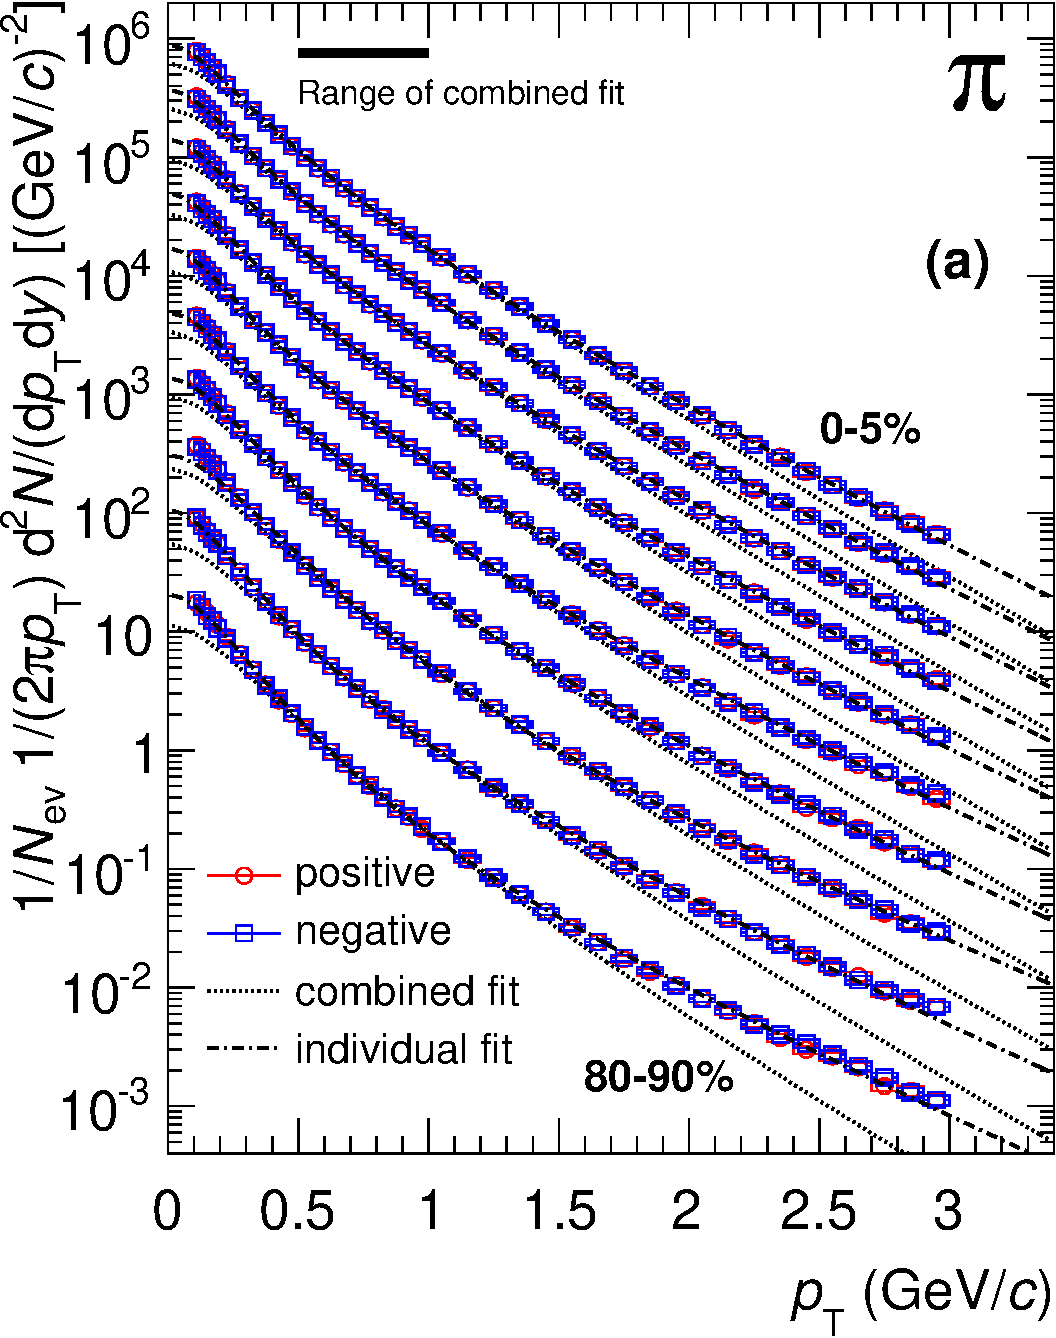
\includegraphics[width=\textwidth]{expdata/alice-spectra-0}
      \column{.3\textwidth}
      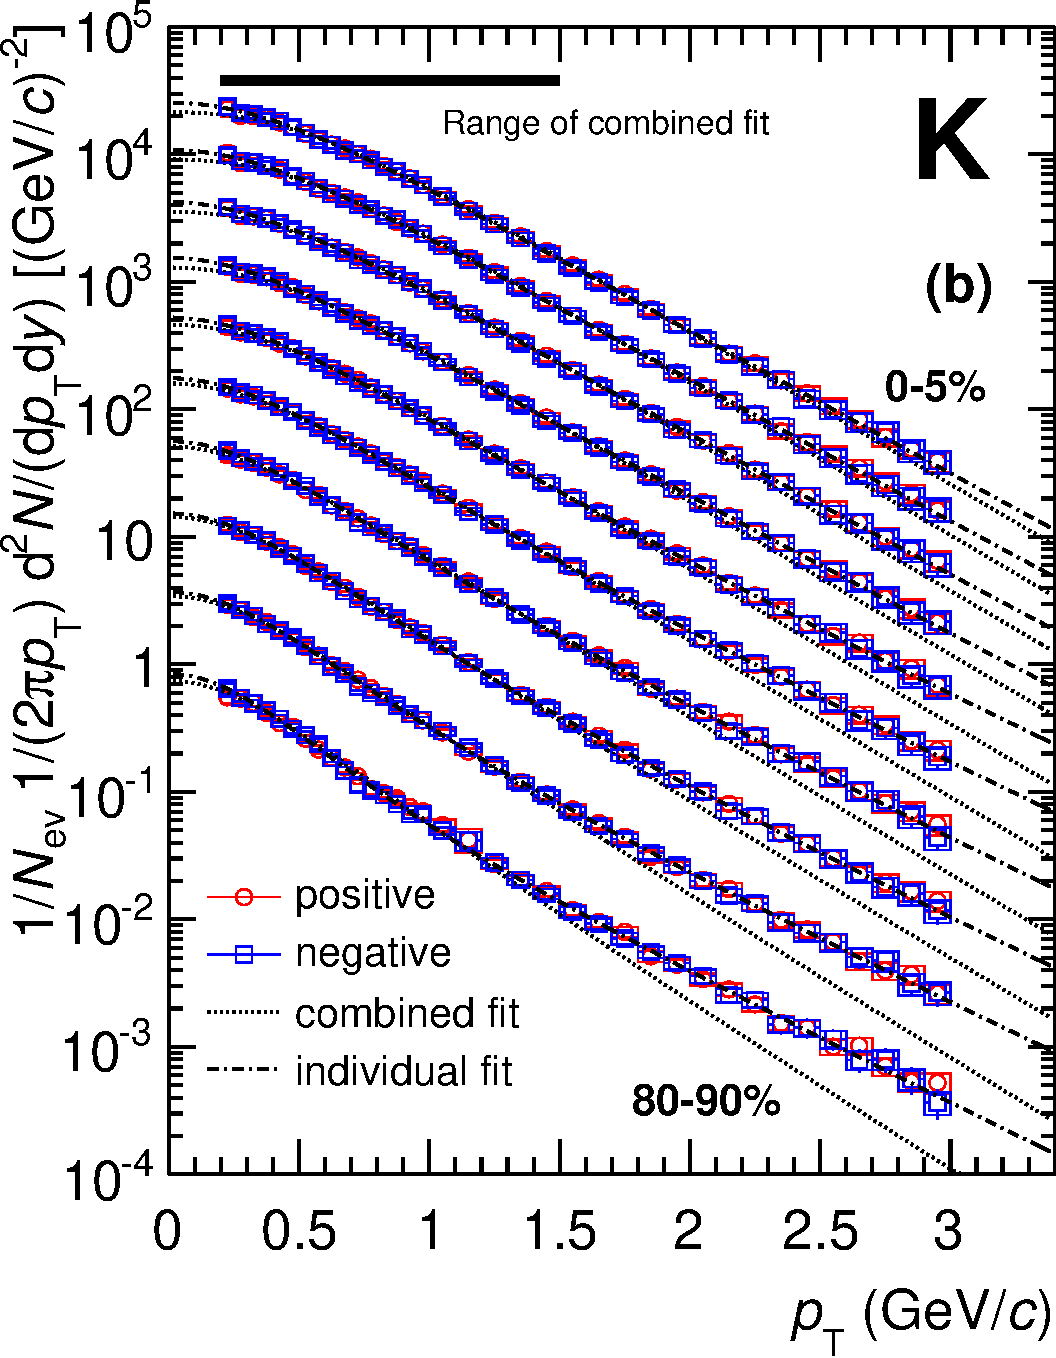
\includegraphics[width=\textwidth]{expdata/alice-spectra-1} \\
      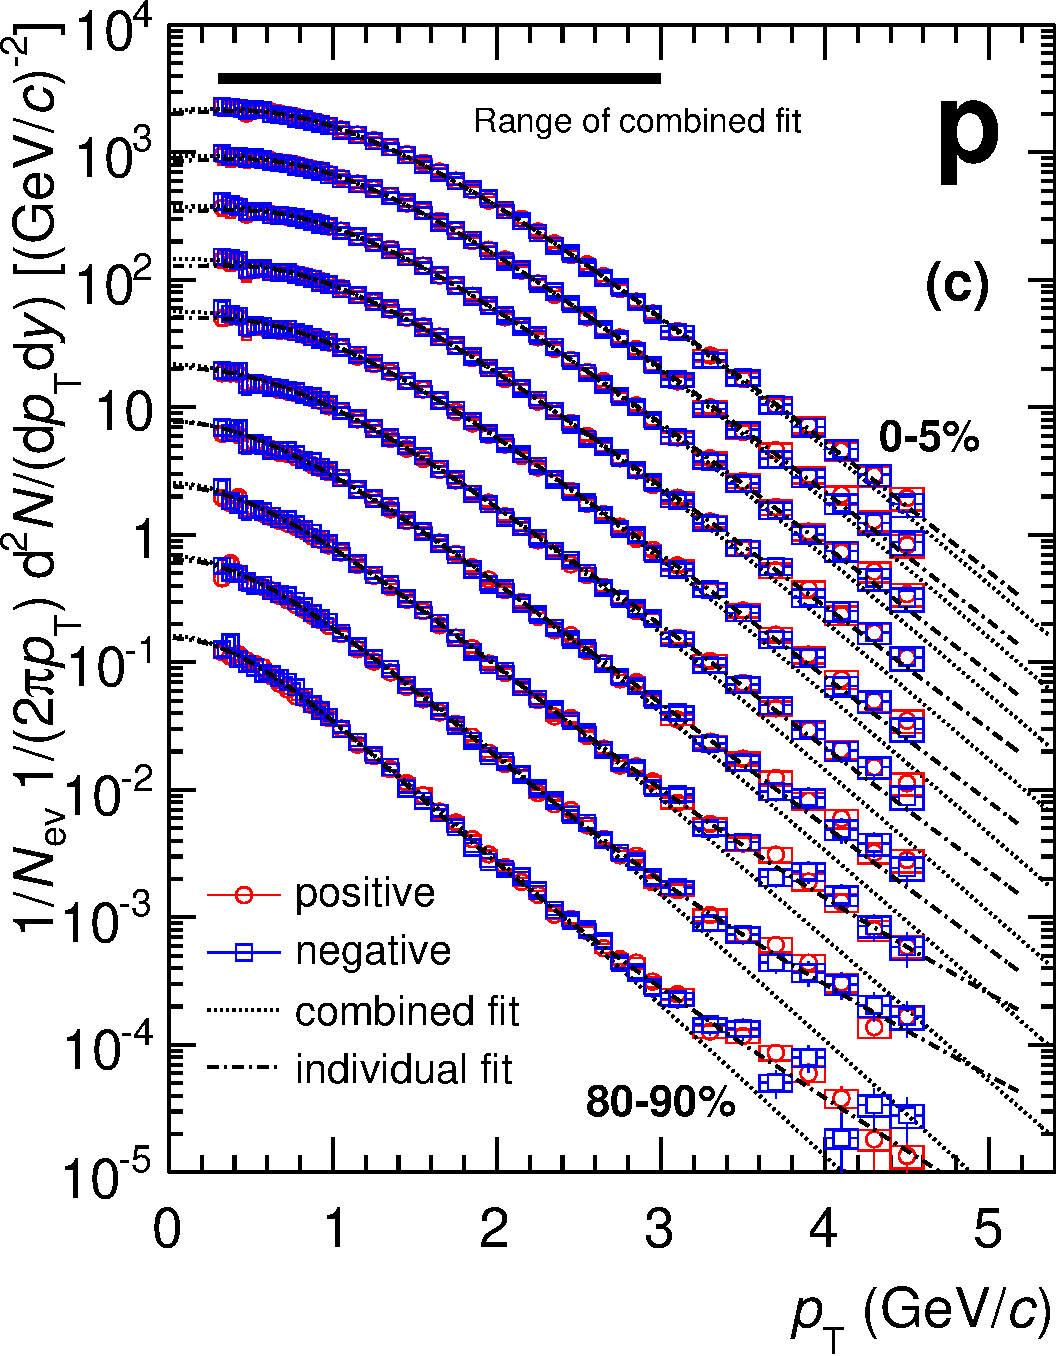
\includegraphics[width=\textwidth]{expdata/alice-spectra-2}
    \end{columns}
    \medskip
    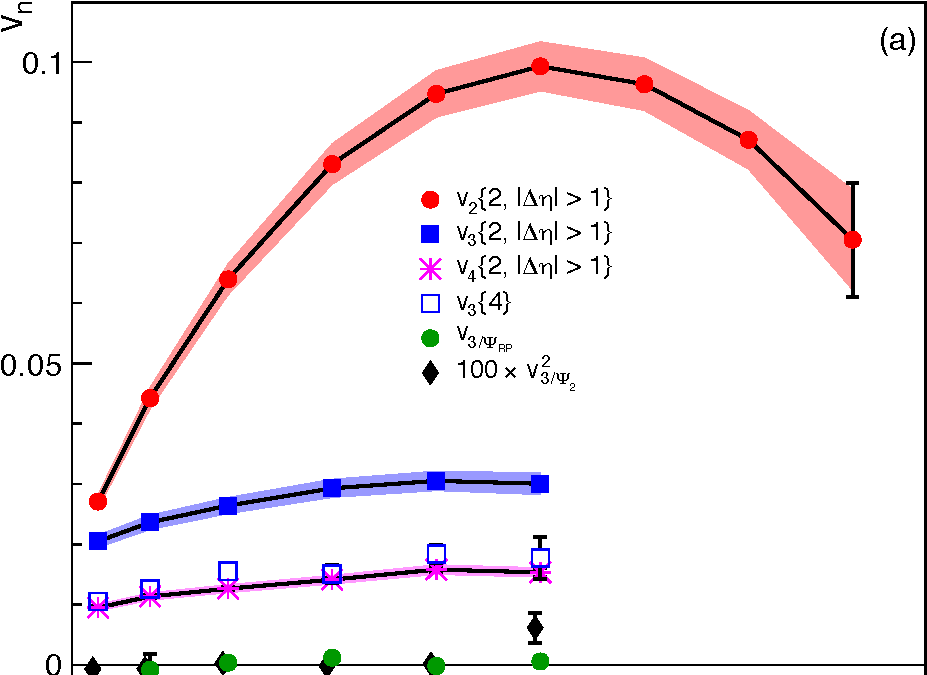
\includegraphics[width=\textwidth]{expdata/alice-flow}
  \end{columns}
  \begin{center}
    All experimental data from the ALICE collaboration at the LHC \\
    Pb-Pb collisions at $\sqrt s = 2.76$ TeV
  \end{center}
\end{frame}

\begin{frame}{Training data}
  \begin{tikzpicture}[remember picture, overlay]
    \node[yshift=-1em] at (current page.center) {
      \includegraphics{observables_prior}
    };
    \node[above left=1em of current page.center, text width=.5\textwidth] {
      \begin{itemize}
        \item Model calculations at each design point
        \item To be used as training data for emulator
      \end{itemize}
    };
  \end{tikzpicture}
\end{frame}

\againframe<4>{flowchart}

\begin{frame}{Gaussian process emulator}
  \vspace{1em}
  \begin{columns}[c]
    \column{.58\textwidth}
    Gaussian process:
    \begin{itemize}
      \item Stochastic function: maps inputs to normally-distributed outputs
      \item Specified by mean and covariance functions
    \end{itemize}
    \bigskip
    As a model emulator:
    \begin{itemize}
      \item Non-parametric interpolation
      \item Predicts \emph{probability distributions}
        \begin{itemize}
          \item Narrow near training points, \\ wide in gaps
        \end{itemize}
      \item Fast surrogate to actual model
    \end{itemize}
    \column{.45\textwidth}
    \includegraphics{gp}
  \end{columns}
\end{frame}

\begin{frame}{Multivariate output}
  \begin{columns}
    \column{.55\textwidth}
    Many highly correlated outputs \\
    $\rightarrow$ \textbf{principal component analysis} \\[1em]
    PCs = eigenvectors of sample covariance matrix
    \begin{equation*}
      Y\tran Y = U \Lambda U\tran
    \end{equation*}
    Transform data into orthogonal, uncorrelated linear combinations
    \begin{equation*}
      Z = \sqrt m \, YU
    \end{equation*}
    Emulate each PC independently
    \column{.45\textwidth}
    \includegraphics<1>{pca}
    \only<2>{\hspace{3em}68 outputs $\rightarrow$ 8 PCs \\[1em]}
    \includegraphics<2>{pca_variance}
  \end{columns}
\end{frame}

\begin{frame}{Validation}
  \begin{center}
    Independent 50-point validation design \\[1em]
    Run full model and predict with emulator
  \end{center}
  \includegraphics{validation}
\end{frame}

\againframe<5>{flowchart}

\newcommand{\st}{_\star}
\newcommand{\ex}{_\text{exp}}

\begin{frame}{Calibration}
  \begin{center}
    Assume true parameters $\xs$ exist $\rightarrow$ find posterior distribution
  \end{center}
  \begin{equation*}
    P(\xs|X,Y,\yexp) \propto P(X,Y,\yexp|\xs) \, P(\xs)
  \end{equation*}
  \begin{center}
    given design $X$, training data $Y$, experimental data $\yexp$
  \end{center}
  \begin{itemize}
    \item Flat prior
    \item Likelihood (in PC space):
      \begin{equation*}
        P(X,Z,\z\ex|\x\st) \propto
        \exp\biggl\{
          -\frac{1}{2} (\z\st - \z\ex)\tran \Sigma_z^{-1} (\z\st - \z\ex)
        \biggr\}
      \end{equation*}
      with flat 10\% uncertainty on PCs
      \begin{equation*}
        \Sigma_z = \text{diag}(\sigma^2_z\,\z\ex), \quad
        \sigma_z = 0.10
      \end{equation*}
  \end{itemize}
\end{frame}

\begin{frame}{MCMC}
  \centering
  \textbf{Markov chain Monte Carlo}
  \vspace{1ex}
  \begin{itemize}
    \item Random walk through parameter space weighted by posterior
    \item Large number of samples \\
      $\rightarrow$ chain equilibrates to posterior distribution
  \end{itemize}
  \vspace{3ex}
  \textbf{This study}
  \vspace{1ex}
  \begin{itemize}
    \item Emulator serves as stand-in for full model
    \item Affine-invariant ensemble sampler: many interdependent walkers
    \item 1000 walkers, $10^6$ burn-in steps, $10^7$ production steps
  \end{itemize}
\end{frame}


\section{Results}

\againframe<6>{flowchart}

\begin{frame}{\only<1>{Training data}\only<2>{Posterior samples}}
  \begin{tikzpicture}[remember picture, overlay]
    \node[yshift=-1em] at (current page.center) {
      \includegraphics<1>{observables_prior}
      \includegraphics<2>{observables_posterior}
    };
    \node[
      below right=4.5em and 2.2em of current page.north west,
      text width=.5\textwidth, align=center
    ] {
      Model calculations at each design point \\
      \only<2->{
        $\downarrow$ \\
        Emulator predictions from calibrated posterior
      }
    };
  \end{tikzpicture}
\end{frame}

\begin{frame}<1>[label=posterior, plain]
  \centering
  \smallskip
  \includegraphics<1-3>{posterior_lower}
  \includegraphics<4>{posterior_pair}
  \begin{tikzpicture}[remember picture, overlay]
    \node<1-3>[below left=1.5em and 3em of current page.north east, color=theme, font=\Large]
    (title) {
      Posterior distribution
    };
    \node<1-3>[below of=title, font=\small, align=left] {
      Estimated values: medians \\
      Uncertainties: 90\% credible intervals
    };
    \node<4>[color={rgb:red,94;green,165;blue,208}, rotate=90, yshift=-2em, font=\Large]
    at (current page.west) {
      Identified particles
    };
    \node<4>[color={rgb:red,218;green,86;blue,78}, rotate=-90, yshift=-2em, font=\Large]
    at (current page.east) {
      Charged particles
    };
  \end{tikzpicture}
\end{frame}

\begin{frame}{Constraining initial conditions}
  \begin{columns}[t]
    \column{.65\textwidth}
    \trento\ ansatz:
    \genmean
    \medskip
    \includegraphics{posterior_p_arrows}
    \column{.35\textwidth}
    \vspace{.7cm}
    \begin{center}
      \small Mimics other models: \\[1em]
      \includegraphics[width=\textwidth]{trento_ecc_compare}
    \end{center}
  \end{columns}
  \begin{itemize}
    \item Entropy deposition approx.\ proportional to geometric mean of nuclear density: $s \sim \sqrt{T_A T_B}$
    \item Confirms success / failure of existing models
  \end{itemize}
\end{frame}

\againframe<2>[plain, noframenumbering]{posterior}

\begin{frame}{Estimate of $(\eta/s)(T)$}
  \begin{center}
    \includegraphics{etas_estimate}
  \end{center}
  \begin{itemize}
    \item First systematic, quantitative estimate of $T$-dependent $\eta/s$
    \item ``Handle'' near 200 MeV $\rightarrow$ need multiple beam energies!
  \end{itemize}
\end{frame}

\againframe<3-4>[plain, noframenumbering]{posterior}

\begin{frame}{Most probable parameters}
  \begin{center}
    \footnotesize
    \begin{tabular}{ll@{\hspace{3em}}ll}
      norm & 120. / 129.    & $\eta/s$ min      & 0.08  \\
      $p$  & 0.0            & $\eta/s$ slope    & 0.85 / 0.75 GeV$^{-1}$  \\
      $k$  & 1.5  / 1.6     & $\zeta/s$ norm    & 1.25 / 1.10 \\
      $w$  & 0.43 / 0.49 fm & $T_\text{switch}$ & 0.148 GeV \\
    \end{tabular}
  \end{center}
  \makebox[\textwidth]{
    \includegraphics<1>{mode_observables_id}
    \includegraphics<2>{mode_observables_both}
  }
\end{frame}


\section{Conclusion}

\begin{frame}{Summary}
  \begin{itemize}
    \item \trento\ parametric initial conditions, viscous relativistic hydrodynamics, hadronic afterburner (UrQMD)
      \smallskip
    \item Excellent simultaneous fit to experimental data
      \smallskip
    \item Estimated initial condition and QGP medium properties
      \begin{itemize}
        \item Entropy deposition $\sim$ geometric mean of nuclear density
        \item Relation between $\eta/s$ min and slope, handle near 200 MeV
        \item Finite bulk viscosity
        \item $T_\text{switch}$ constrained by particle ratios only
      \end{itemize}
      \bigskip
    \item Additional beam energies (200 GeV, 2.76 TeV, 5.02 TeV)
    \item Improve treatment of uncertainty
  \end{itemize}
\end{frame}


\appendix


\begin{frame}{Gaussian processes}
  \begin{definition}
    A Gaussian process is a collection of random variables, any finite number of which have a joint Gaussian distribution.
  \end{definition}
  \medskip
  Stochastic function: $\x \rightarrow y$ \\
  \begin{itemize}
    \item $\x$ = $n$-dimensional input vector
    \item $y$ = normally distributed output
  \end{itemize}
  Specified by
  \begin{itemize}
    \item Mean function $\mu(\x)$
    \item Covariance function $\sigma(\x, \x')$, e.g.:
      \begin{equation*}
        \sigma(\x, \x') = \exp\biggl( -\frac{|\x - \x'|^2}{2\ell^2} \biggr)
      \end{equation*}
  \end{itemize}
\end{frame}

\begin{frame}{Conditioning a Gaussian process}
  Given
  \begin{itemize}
    \item training input points $X$ and
    \item observed training outputs $\y$ at $X$
  \end{itemize}
  the predictive distribution at arbitrary test points $X_*$ is the multivariate-normal distribution
  \begin{align*}
    \y_* &\sim \mathcal N(\boldsymbol\mu, \Sigma), \\
    \boldsymbol\mu &= \sigma(X_*, X)\sigma(X, X)^{-1}\y, \\
    \Sigma &= \sigma(X_*,X_*) - \sigma(X_*,X)\sigma(X,X)^{-1}\sigma(X,X_*).
  \end{align*}
\end{frame}


\end{document}
